\documentclass[tikz,border=6pt]{standalone}
\usepackage[T1]{fontenc}
\usepackage[scaled=0.92]{helvet}
\usepackage{amsmath,amssymb}
\usepackage{tikz}
\usetikzlibrary{arrows.meta,positioning,shapes.geometric,calc}

\begin{document}
\sffamily
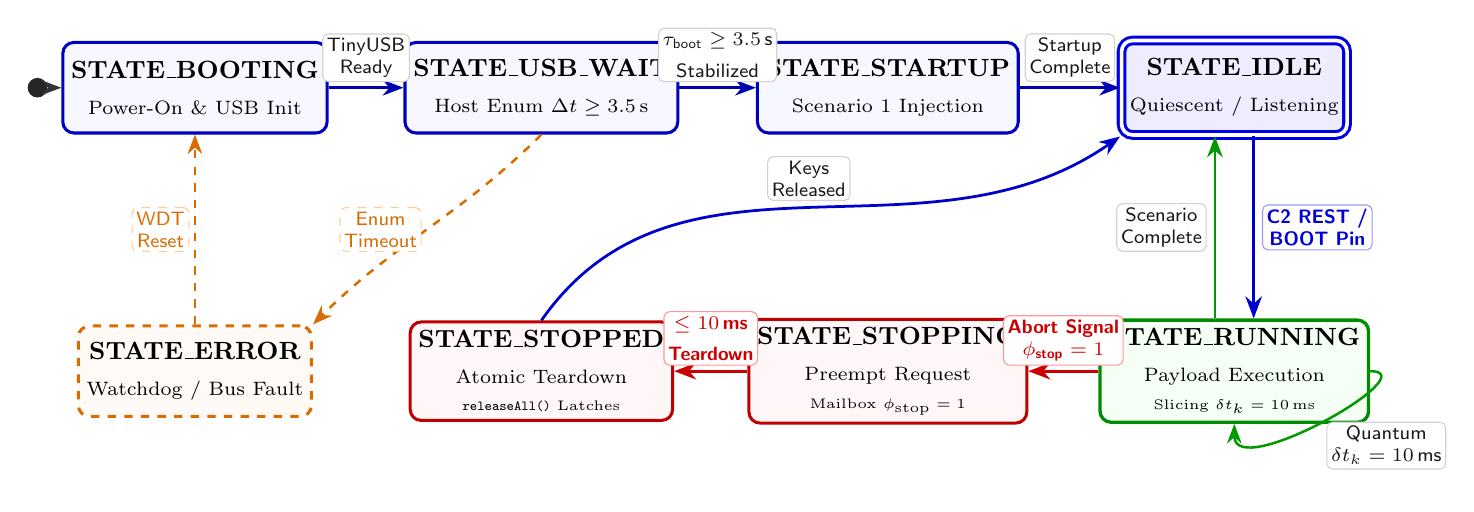
\begin{tikzpicture}[
    >=Stealth,
    font=\small,
    % Standard Operational State
    st_norm/.style={
        rectangle,
        rounded corners=4pt,
        draw=blue!75!black,
        line width=1.1pt,
        fill=blue!3!white,
        minimum width=2.45cm,
        minimum height=1.15cm,
        inner sep=3pt,
        align=center
    },
    % Idle State (Double Border Hub)
    st_idle/.style={
        rectangle,
        rounded corners=4pt,
        draw=blue!90!black,
        double,
        double distance=1.3pt,
        line width=1.1pt,
        fill=blue!7!white,
        minimum width=2.55cm,
        minimum height=1.2cm,
        inner sep=3pt,
        align=center
    },
    % Active Running State
    st_run/.style={
        rectangle,
        rounded corners=4pt,
        draw=green!55!black,
        line width=1.2pt,
        fill=green!4!white,
        minimum width=2.55cm,
        minimum height=1.15cm,
        inner sep=3pt,
        align=center
    },
    % Emergency Preempt / Stop States
    st_stop/.style={
        rectangle,
        rounded corners=4pt,
        draw=red!75!black,
        line width=1.1pt,
        fill=red!3!white,
        minimum width=2.45cm,
        minimum height=1.15cm,
        inner sep=3pt,
        align=center
    },
    % Error / Fault State
    st_err/.style={
        rectangle,
        rounded corners=4pt,
        draw=orange!85!black,
        line width=1.1pt,
        dashed,
        fill=orange!4!white,
        minimum width=2.45cm,
        minimum height=1.15cm,
        inner sep=3pt,
        align=center
    },
    % Edge Badges
    lbl/.style={
        font=\sffamily\scriptsize,
        fill=white,
        draw=gray!35,
        line width=0.4pt,
        rounded corners=2pt,
        inner sep=1.5pt,
        align=center,
        text=black!90
    },
    lbl_blue/.style={
        font=\sffamily\scriptsize\bfseries,
        fill=white,
        draw=blue!40,
        line width=0.4pt,
        rounded corners=2pt,
        inner sep=1.5pt,
        align=center,
        text=blue!85!black
    },
    lbl_red/.style={
        font=\sffamily\scriptsize\bfseries,
        fill=white,
        draw=red!40,
        line width=0.4pt,
        rounded corners=2pt,
        inner sep=1.5pt,
        align=center,
        text=red!80!black
    },
    lbl_amber/.style={
        font=\sffamily\scriptsize,
        fill=white,
        draw=orange!40,
        line width=0.4pt,
        rounded corners=2pt,
        inner sep=1.5pt,
        align=center,
        text=orange!85!black
    }
]

% Start Token
\node[circle, fill=black!85, inner sep=2.5pt] (start) at (0.1, 1.8) {};

% ==============================================================================
% 4-COLUMN SYMMETRIC GRID: Top Row (Init -> Idle) at y = 1.8
% ==============================================================================
\node[st_norm] (boot)    at (2.1, 1.8)  {\textbf{STATE\_BOOTING}\\[2pt]\scriptsize Power-On \& USB Init};
\node[st_norm] (usbwait) at (6.5, 1.8)  {\textbf{STATE\_USB\_WAIT}\\[2pt]\scriptsize Host Enum $\Delta t \ge 3.5$\,s};
\node[st_norm] (startup) at (10.9, 1.8) {\textbf{STATE\_STARTUP}\\[2pt]\scriptsize Scenario 1 Injection};
\node[st_idle] (idle)    at (15.3, 1.8) {\textbf{STATE\_IDLE}\\[2pt]\scriptsize Quiescent / Listening};

% ==============================================================================
% 4-COLUMN SYMMETRIC GRID: Bottom Row (Fault & Teardown) at y = -1.8
% ==============================================================================
\node[st_err]  (error)    at (2.1, -1.8)  {\textbf{STATE\_ERROR}\\[2pt]\scriptsize Watchdog / Bus Fault};
\node[st_stop] (stopped)  at (6.5, -1.8)  {\textbf{STATE\_STOPPED}\\[2pt]\scriptsize Atomic Teardown\\[-1pt]\tiny \texttt{releaseAll()} Latches};
\node[st_stop] (stopping) at (10.9, -1.8) {\textbf{STATE\_STOPPING}\\[2pt]\scriptsize Preempt Request\\[-1pt]\tiny Mailbox $\phi_{\text{stop}}=1$};
\node[st_run]  (running)  at (15.3, -1.8) {\textbf{STATE\_RUNNING}\\[2pt]\scriptsize Payload Execution\\[-1pt]\tiny Slicing $\delta t_k = 10$\,ms};

% ==============================================================================
% Top Row Transitions (Spacing: 4.4cm, gap: 1.95cm)
% ==============================================================================
\draw[->, line width=0.9pt, draw=black!80] (start) -- (boot);
\draw[->, line width=1.0pt, draw=blue!70!black] (boot) -- node[above=2pt, lbl] {TinyUSB\\Ready} (usbwait);
\draw[->, line width=1.0pt, draw=blue!70!black] (usbwait) -- node[above=2pt, lbl] {$\tau_{\text{boot}} \ge 3.5$\,s\\[3.5pt]Stabilized} (startup);
\draw[->, line width=1.0pt, draw=blue!70!black] (startup) -- node[above=2pt, lbl] {Startup\\Complete} (idle);

% ==============================================================================
% Column 4 Inter-Row: IDLE <-> RUNNING
% ==============================================================================
\draw[->, line width=1.1pt, draw=blue!80!black] ([xshift=7pt]idle.south) -- node[pos=0.5, right=3pt, lbl_blue] {C2 REST /\\BOOT Pin} ([xshift=7pt]running.north);
\draw[->, line width=1.0pt, draw=green!60!black] ([xshift=-7pt]running.north) -- node[pos=0.5, left=3pt, lbl] {Scenario\\Complete} ([xshift=-7pt]idle.south);

% Cooperative slicing loop on RUNNING
\draw[->, line width=0.9pt, draw=green!60!black] (running.east) .. controls +(right:0.75cm) and +(down:0.75cm) .. node[below right=1pt, lbl] {Quantum\\$\delta t_k = 10$\,ms} (running.south);

% ==============================================================================
% Bottom Row Transitions: RUNNING -> STOPPING -> STOPPED
% ==============================================================================
\draw[->, line width=1.1pt, draw=red!80!black] (running) -- node[above=2pt, lbl_red] {Abort Signal\\$\phi_{\text{stop}}=1$} (stopping);
\draw[->, line width=1.1pt, draw=red!80!black] (stopping) -- node[above=2pt, lbl_red] {$\le 10$\,ms\\[3.5pt]Teardown} (stopped);

% Return transition from STOPPED back to IDLE
\draw[->, line width=1.0pt, draw=blue!80!black] (stopped.north) to[out=55, in=215] node[pos=0.5, above=2pt, lbl] {Keys\\Released} (idle.south west);

% ==============================================================================
% Column 1 & 2 Error & Recovery Transitions
% ==============================================================================
\draw[->, line width=0.9pt, dashed, draw=orange!85!black] (usbwait.south) to[out=-135, in=45] node[pos=0.5, left=2pt, lbl_amber] {Enum\\Timeout} (error.north east);
\draw[->, line width=0.9pt, dashed, draw=orange!85!black] (error.north) -- node[left=2pt, lbl_amber] {WDT\\Reset} (boot.south);

\end{tikzpicture}
\end{document}
